\chapter{Random Forest}
\section{Alberi Binari}
Gli alberi binari sono un strttura dati in cui ogni nodo padre ha messo due nodi figli, destro e sinistro. \\
I nodi si dividono in:
\begin{itemize}
  \item \textbf{Split nodes:} nodi di decisione.
  \item \textbf{Leaf nodes:} nodi finali con la soluzione.
\end{itemize}
Inoltre, ci sono alcuni parametri importanti da considerare:
\begin{itemize}
  \item \textbf{Vettore di feature:} $v \in \mathbb{R}^N$.
  \item \textbf{Funzione di split:} $f_n(v) : \mathbb{R} \rightarrow \mathbb{R}^N$.
  \item \textbf{Thresholds:} $t_n \in \mathbb{R}$.
  \item \textbf{Classificazione:} $P_n(c)$.
\end{itemize}
Ogni decisione presa nell'albero rappresenta una retta.

\begin{figure}[!htb]
    \centering
    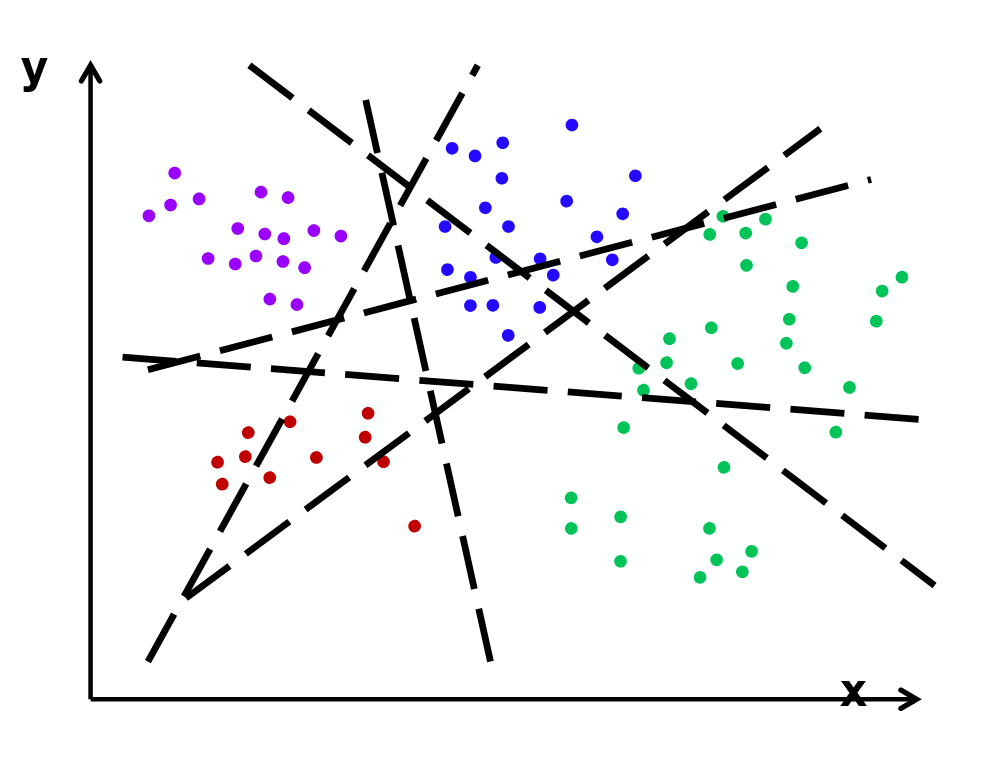
\includegraphics[width=0.4\linewidth]{Images/random_forest/graph.png}
    \caption{Dimostrazione grafica delle scelte in un albero.}
\end{figure}

\section{Ottimizzazione}
Per prima cosa bisogna definire le due label, destra e sinistra:
\begin{enumerate}
  \item \textbf{Left split:} $I_l = \{i \in I_n \mid f(v_i) < t\}$.
  \item \textbf{Right split:} $I_r = I_n / I_l$.
\end{enumerate}
Dove $t \in (\min_i f(v_i), \max_i f(v_i))$.
L'obiettievo è massimizzare l'\textbf{information gain}, scegliendo correntamente la funzione $f$ e il threshold $t$.
Per fare questo, è necessario minimizzare l'entropia, che si calcola come:
\[
  E = - \sum^{nLabels}_i{h_i \log_2{(h_i)}}
\]
Ottenendo:
\[
  \Delta E = -\frac{|I_l|}{|I_n|} E(I_l) - \frac{|I_r|}{|I_n|} E(I_r)
\]
\begin{note}[Qaunte feature e threshold usare?]
  Ci sono diversi casi:
  \begin{itemize}
    \item \textbf{Solo uno:} sarebbe troppo randomico.
    \item \textbf{Pochi:} addestramento rapido ma rischio di underfitting e forse eccessiva profondità.
    \item \textbf{Tanti:} addestramento più lento e possibile overfitting.
  \end{itemize}
\end{note}

\section{Foresta}
Una foresta è un insieme di alberi decisionali.\\
Utilizziamo la media delle classificazioni con alberi decisionali.
La classificazione risulta una normalizzazione rispetto al numero di alberi:
\[
  P(c|v) = \frac{1}{T} \sum_{t=1}^T P_t(c|v)
\]
Ci sono tre tipi di foreste:
\begin{enumerate}
  \item \textbf{Classificazione}, massimizzare l'information gain:
    \[
      I = H(S) - \sum_{i=1}^2 \frac{|S_i|}{|S|} H(S_i)
    \]
    Serve a clasfficare le classi.
  \item \textbf{Regressione}, massimizzare l'information gain:
    \[
      Err(S) - \sum_{i=1}^2 \frac{|S_i|}{|S|} Err(S_i)
    \]
    Dove:
    \[
      Err(S) = \sum_{j \in S} (y_j - y(x_j))^2
    \]
    Serve per predire valori reali.
  \item \textbf{Clustering}, ci sono due possibilità, minimizzare l'\textbf{imbalance}:
    \[
      B = |\log|S_1| - \log|S_2||
    \]
    Oppure massimizzare la likelyhood della Gaussiana:
    \[
      T = |\Lambda_S| - \sum_{i=1}^2 \frac{|S_i|}{|S|} |\Lambda_{S_i}|
    \]
    Serve per predire una somiglianza fra classi.
\end{enumerate}
